\documentclass[conference]{IEEEtran}
\IEEEoverridecommandlockouts
% The preceding line is only needed to identify funding in the first footnote. If that is unneeded, please comment it out.
\usepackage{cite}
\usepackage{amsmath,amssymb,amsfonts}
\usepackage{algorithmic}
\usepackage{graphicx}
\usepackage[utf8]{inputenc}
\usepackage{textcomp}
\usepackage[english,ngerman,brazilian]{babel}
\def\BibTeX{{\rm B\kern-.05em{\sc i\kern-.025em b}\kern-.08em
    T\kern-.1667em\lower.7ex\hbox{E}\kern-.125emX}}
\begin{document}

\title{Projeto Demonstrativo 2 - Calibração de Câmeras}

\author{\IEEEauthorblockN{Frederico Guth (18/0081641)}
\IEEEauthorblockA{\textit{Tópicos em Sistemas de Computação, ,} \\
\textit{Turma TC - Visão Computacional (PPGI)}\\
\textit{Universidade de Brasília}\\
Brasília, Brasil\\
fredguth@fredguth.com}
}

\maketitle

\begin{abstract}
This document is a model and instructions for \LaTeX.
This and the IEEEtran.cls file define the components of your paper [title, text, heads, etc.]. *CRITICAL: Do Not Use Symbols, Special Characters, Footnotes, 
or Math in Paper Title or Abstract.
\end{abstract}

\begin{IEEEkeywords}
component, formatting, style, styling, insert
\end{IEEEkeywords}

\section{Introdução}
Uma câmera é um instrumento de aquisição de imagens. Conhecendo seus parâmetros intrínsecos, como distância focal e distorção da lente, e extrínsecos, sua rotação e translação no sistema de coordenadas do mundo real, é possível estimar a posição 3D de um objeto a partir de sua imagem\cite{tese}, o que possibilita diversas aplicações: por exemplo, a mensuração da altura de pessoas registradas em vídeos de camêras de segurança ou a estimativas de posições de atletas em campo, entre outras.

\subsection{Objetivos}
Os objetivos deste projeto são a aplicação prática da teoria de calibração de câmeras e o desenvolvimento de uma "régua visual", capaz de medir um objeto através da sua imagem.

\section{Revisão Teórica}
Os objetivos deste projeto são a aplicação prática da teoria de calibração de câmeras e o desenvolvimento de uma "régua visual", capaz de medir um objeto através da sua imagem.

\subsection{Modelo de Câmera com Coordenadas Homogêneas}
O modelo de câmera estenopeica (pinhole) faz um mapeamento geométrico do mundo 3D para o plano da imagem 2D.\cite{unicamp}

\begin{figure}[h!]
\begin{center}
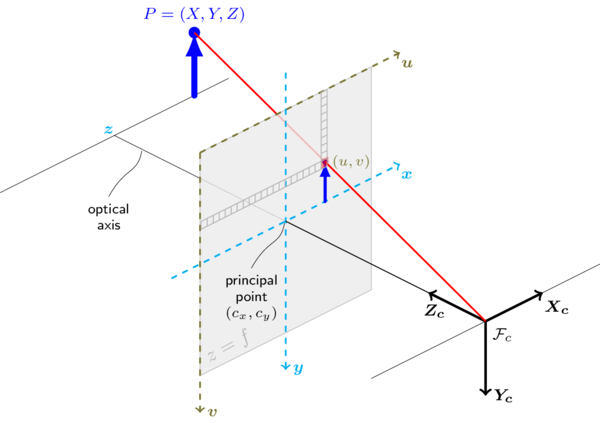
\includegraphics[width=0.5\columnwidth]{pinhole.png}
\caption{Imagem do arquivo venn.jpg}
\end{center}
\end{figure}

Se os pontos do mundo (X) e da imagem (x) são representados por coordenadas homogêneas, podemos expressar matematicamente a projeção da câmera como uma matriz\cite{tese}:

\[\lambda \cdot x = P \cdot X\]

onde \(\lambda\) é um fator de escala e P é a matriz 3x4 de projeção, também chamada matriz de calibração.

Sendo X expresso em coordenadas euclidianas, P pode ser decomposto em duas entidades geométricas: os parâmetros intrísecos e extrísecos de calibração\cite{tese}

\[P = K (R\cdot t)\] 
\[t = -R \cdot \widetilde{C}\]
onde \(\widetilde{C}\) é a origem da imagem. \cite{Hartley2004}

Os parâmetros intrísecos de calibração descrevem a transformação entre a imagem ideal e a imagem em pixels
$$
K = \begin{pmatrix} 
f & s & u_0 \\
0 & \alpha f & v_0\\
0 & 0 & 1
\end{pmatrix}
$$
e os extrínsecos são a rotação e translação que transformam pontos no espaço do objeto para pontos no espaço da imagem e vice-versa\cite{tese}.

Como há 6 graus de liberdade nos parâmetros extrínsecos e 5 nos intrísecos, é necessário pelo menos 6 correspondências \({x_i \leftrightarrow X_i}\) do mesmo ponto no espaço da imagem e no espaço do objeto para obter P\cite{tese}. 

Como há um erro inerente nas medidas experimentais, para melhorar a qualidade da estimativa é preciso usar \(n > 6\) correspondências (como será visto na Metodologia, usaremos 48). Como não há uma única matriz P que resolve esse sistema de equações é adicionar restrições.  

Um método comum é adicionar a restrição \(p_34 = 0\)\cite{Hartley2004, tese}, mas uma melhor abordagem\cite{tese} é fazer a minimização do somatório da distância euclidiana entre o ponto observado e o estimado.

A biblioteca OpenCV\cite{OpenCV} usa essa última abordagem e aplica o método Levenberg-Marquant para resolver a minimização. 

\subsection{Distorções}

O modelo até aqui descrito descreve uma câmera ideal, mas as lentes das câmeras reais podem gerar distorções.  Essas distorções também são parâmetros intrínsecos que precisam ser considerados. 

A distorção radial causa uma curvatura no mapeamento de retas\cite{unicamp}.
(inserir imagem distorção)

A correção dessa distorção pode ser modelada da seguinte maneira: 

    \[x_{retificado} = x( 1 + k_1 r^2 + k_2 r^4 + k_3 r^6)\]
    \[y_{retificado} = y( 1 + k_1 r^2 + k_2 r^4 + k_3 r^6)\]

Outra distorção comum é a tangencial, que ocorre quando o plano da lente não está alinhado perfeitamente em paralelo ao plano da imagem. Para corrigir:


\[x_{retificado} = x + [ 2p_1xy + p_2(r^2+2x^2)] \]
\[y_{retificado} = y + [ p_1(r^2+ 2y^2)+ 2p_2xy] \]


Esses cinco parâmetros são conhecidos como coeficientes de distorção
\((k_1 \hspace{10pt} k_2 \hspace{10pt} p_1 \hspace{10pt} p_2 \hspace{10pt} k_3)\).

% [opencv-camera calibration]
\section{Metodologia}
O modelo da câmera e seus parâmetros foram descritos na seção de Revisão Teórica. Nesta seção, descreve-se como estimá-los experimentalmente.

\subsection{Materiais}
Foram utilizados o seguintes materiais:
\begin{itemize}
\item Uma tábua de compensado
\item Papel contact
\item Um padrão de calibração xadrez impresso em papel A4
\item Uma trena
\item Uma régua
\item Computador MacBook Pro (Retina, 13-inch, Early 2015), Processador Intel Core i5 2,7 GHz, 8GB de RAM
\item Python 3.6.3 :: Anaconda custom (64-bit)
\item OpenCV 3.4.0
\end{itemize}

\subsection{Preparação}
 \begin{enumerate}
 \item Imprime-se o padrão de calibração em folha A4 e o cola à tábua de compensado usando o Papel contact
 \item Com o programa \textit{requisito1.py}, abre-se uma imagem jpg e com cliques do mouse desenha-se um segmento de reta sobre a imagem entre o primeiro e o segundo clique, registrando-se a distância \(||p2 - p1||_2 \) na própria imagem aberta. 
 \end{enumerate}
\subsection{Obtenção dos parâmetros intrínsecos}
 \begin{enumerate}
  \item Com o programa \textit{requisito2.capturate.py}, capturou-se sequências de imagens de um padrão de calibração, como o onipresente tabuleiro de xadrez, em diversas orientações e posições. Foram capturadas mais de cinco sequencias, em diferentes distâncias e cada sequencia apresentava mais de dez imagens. Essas sequencias são gravadas pelo próprio programa em diferentes diretórios. 
  \item Com o programa \textit{requisito2.calibrate.py}, os cantos dos quadrados do padrão de calibração xadrez são detectados e apenas com esses pontos já é possível obter os parâmetros intrínsecos K e os coeficientes de distorção.
 Executamos a calibração para as diversas sequencias de imagens do passo anterior. Os parâmetros intrínsecos e coeficientes de distorção foram armazenados em arquivos xml nos respectivos diretórios.
\item Dado que já temos os coeficientes de distorção, com o programa \textit{requisito2.measure.py} retificamos as imagens da câmera e permitimos medir distâncias na imagem retificada em pixels. 
\end{enumerate}
\subsection{Obtenção dos parâmetros extrínsecos}
\begin{enumerate}
\item Com o programa \textit{requisito3.py}Computamos a correspondencia entre pontos da imagem e do espaço do objeto, atribuindo como origem do sistema de coordenadas do mundo, o ponto de intersecção do canto superior esquerdo. Os parâmetros extrínsecos R e t são obtidos usando a função \textit{solvePnPRansac} da OpenCV.
\item Executamos o passo anterior em três diferentes distâncias, o mais perto possível, o mais longe possível e uma medida intermediária. Medimos a distância da câmera à origem do padrão de calibração usando a trena. Para cada distância, obtemos três vezes os valores de R e t.
\end{enumerate}
\subsection{Obtenção da altura de um objeto através da sua imagem}
Com os parâmetros intrínsecos e extrínsecos,  é possível medir um objeto no mundo real a partir da sua imagem. Neste projeto, entretanto, não se obteve êxito em desenvolver essa funcionalidade no programa \textit{requisito4.py}

\section{Resultados}
\subsection{Medição em pixels de segmentos de imagens}
\subsection{Obtenção dos parâmetros intrínsecos}
\subsection{Obtenção dos parâmetros extrínsecos}

\section{Discussão e Conclusões}
% \begin{table}[htbp]
% \caption{Table Type Styles}
% \begin{center}
% \begin{tabular}{|c|c|c|c|}
% \hline
% \textbf{Table}&\multicolumn{3}{|c|}{\textbf{Table Column Head}} \\
% \cline{2-4} 
% \textbf{Head} & \textbf{\textit{Table column subhead}}& \textbf{\textit{Subhead}}& \textbf{\textit{Subhead}} \\
% \hline
% copy& More table copy$^{\mathrm{a}}$& &  \\
% \hline
% \multicolumn{4}{l}{$^{\mathrm{a}}$Sample of a Table footnote.}
% \end{tabular}
% \label{tab1}
% \end{center}
% \end{table}

% \begin{figure}[htbp]
% \centerline{
\includegraphics{fig.jpg}}
% \caption{Example of a figure caption.}
% \label{fig}
% \end{figure}

\selectlanguage{brazilian}
\bibliographystyle{IEEEtran}
\bibliography{references}

\end{document}
